\subsection{PCIe}
\label{subsec:interconnect-sc-background-pcie}

Peripheral component interconnect express (PCIe) is a high-speed, low-latency packet-based communication protocol that connects peripherals like GPUs, FPGAs, storage devices, and networking devices to the CPU. 
To support high bandwidth and low latency, PCIe supports multiple lanes, where each lane can send data in both directions.
Most PCIe implementations support 1, 2, 4, 8, or 16 lanes, represented as PCIe x1 - x16
\footnote{PCIe x32 exists but is rarely utilised in commercial systems.}.

The PCIe standard has evolved through multiple generations, each offering increased data transfer rates and improved efficiency for computing, networking, and storage applications.
Each major revision of the PCIe standard doubles the bandwidth supported by PCIe.
As such, while PCIe 3.0 x16 supports 16 Gbps, PCIe 4.0 x16 doubles it to 32 Gbps, and PCIe 5.0 doubles it further to 64 Gbps.
While PCIe 6.0 continues this trend, it also adds many newer features, such as 256B FLIT mode, ensuring that each packet is exactly 256 bytes, allowing for deterministic processing and Forward Error Correction (FEC).
PCIe 6.0 also introduces data encryption for data in transit on the PCIe interconnect
\footnote{Very few PCIe 5.0 devices are currently available in the market, and PCIe 6.0 is unavailable}.

As PCIe protocol enables communication between the CPU and peripherals, it requires hardware support from the CPU in the form of the CPU's PCIe root complex.
However, as the PCIe root complex resides on the CPU die, providing an arbitrarily large number of PCIe lanes originating from the CPU to support an arbitrarily large number of peripheral devices becomes challenging.
To alleviate this problem, PCIe utilises either a PCIe Switch or a platform controller hub (PCH) to form a tree-like topology.
A PCIe switch has one upstream port that connects to either the CPU's root complex or another PCIe switch but has multiple downstream ports, each of which can consist of more PCIe switches or endpoints to connect the peripherals.
A PCH is usually integrated within the CPU and provides PCIe access to slower endpoints such as storage, USB ports, and slow network cards such as the one built into the motherboard.

\begin{figure}[!htb]
    \centering
    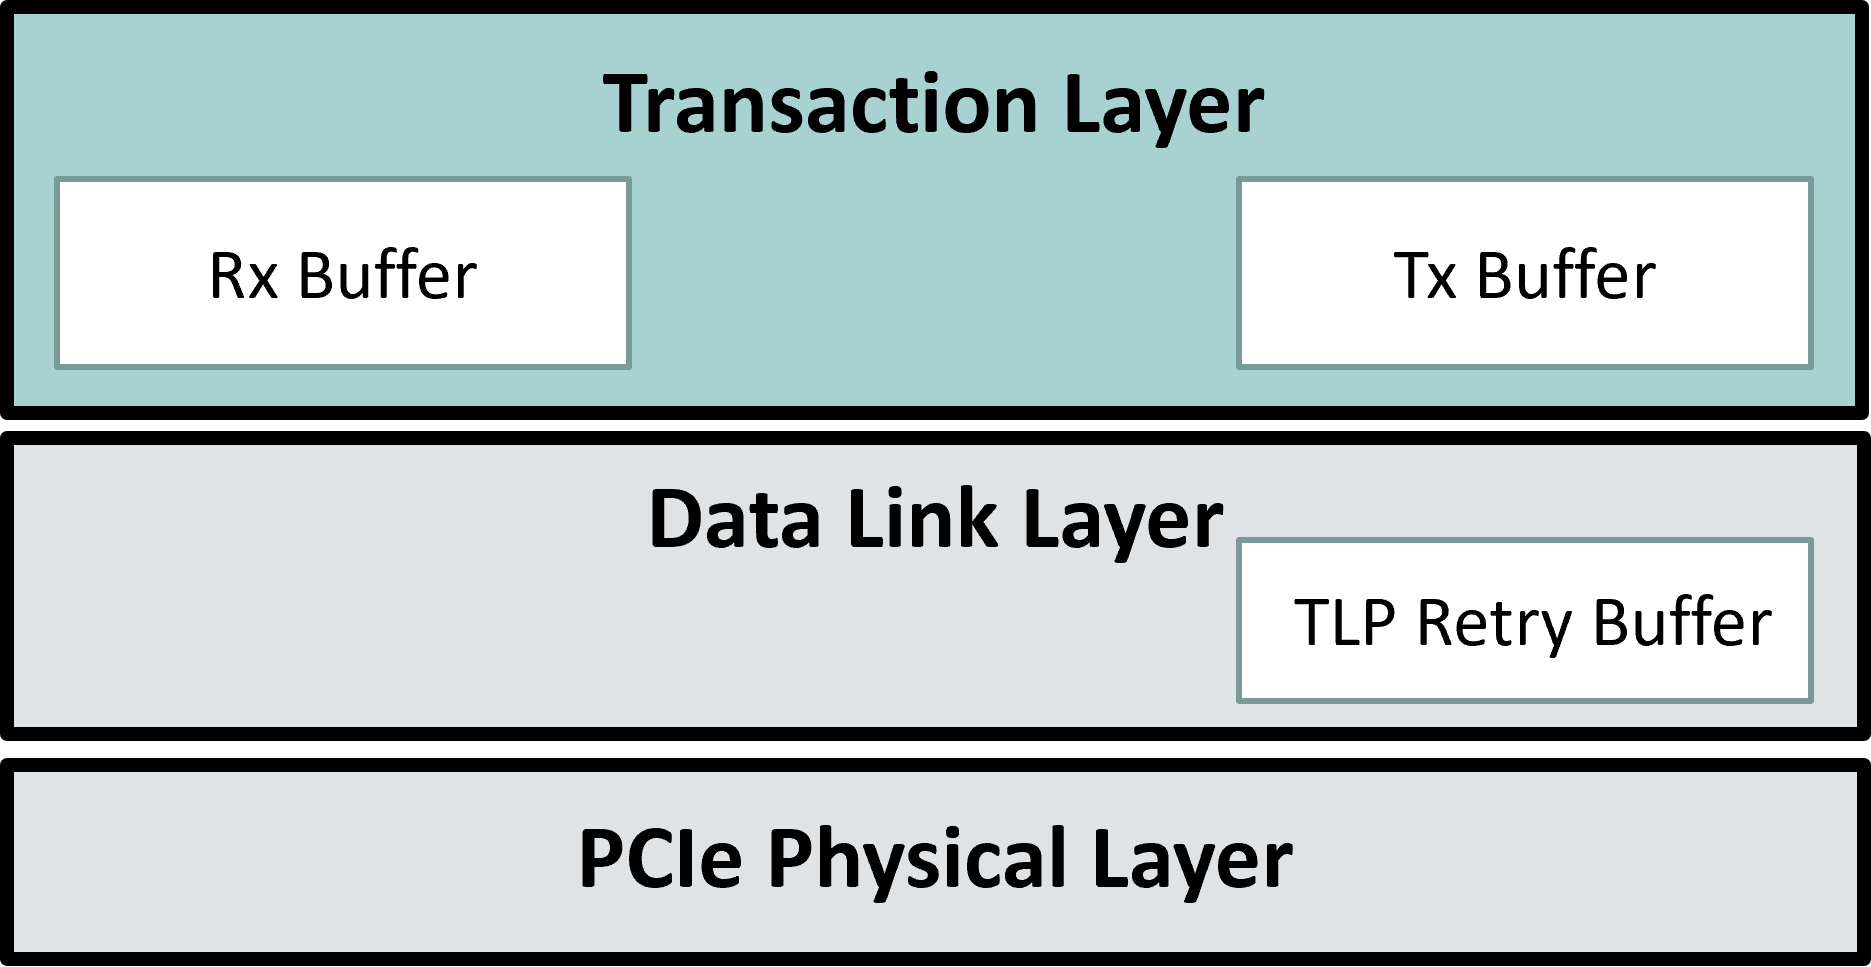
\includegraphics[width=\columnwidth]{figures/interconnect-sc/pcie-controller.png}
    \caption{Simplified PCIe controller}
    \label{fig:pcie-controller}
\end{figure}

Like network protocols, PCIe utilises a layered architecture consisting of the transaction, data link, and physical layers, which are implemented in a PCIe controller (see \Cref{fig:pcie-controller}).
PCIe provides reliable transfer semantics in the data link layer, which relies on cyclic redundancy check (CRC) to detect errors and uses acknowledgements (ACKs) or negative acknowledgements (NACKs) to inform the sender to re-transmit failed packets.
The transaction layer of PCIe supports a fixed set of transactions (see \Cref{tab:pcie-transaction-types}), each of which is one of the following three types:
\textbf{Posted:} Transactions where no response is issued or expected. 
\textbf{Non-posted:} Transactions where a response is required. 
\textbf{Completions:} The response of a previous non-posted transaction.
PCIe enforces strict ordering rules for each type, which we outline in \Cref{tab:pcie-transaction-ordering-rules}.

\begin{table}[!htb]
    \centering
    \begin{tabular}{|l|l|p{0.65\textwidth}|}
        \hline
        \textbf{Transaction} & \textbf{Type} & \textbf{Description} \\ 
        \hline
        Memory Read  & Non-Posted & Read from a memory-mapped address space \\ 
        Memory Write & Posted     & Write to a memory-mapped address space  \\ 
        I/O Read     & Non-Posted & (Legacy PCI) Read from the I/O address space \\ 
        I/O Write    & Non-Posted & (Legacy PCI) Write to the I/O address space \\ 
        Config Read  & Non-Posted & Read control and status registers of the PCIe interface \\ 
        Config Write & Non-Posted & Write control and status registers of the PCIe interface \\  
        Message      & Posted     & Conveys additional information (e.g. Interrupts, Power Management, Error Signalling, Vendor-defined messaging). \\
        Completion   & Completion & Response to all non-posted transactions \\ 
        \hline
    \end{tabular}
    \caption{PCIe transaction types}
    \label{tab:pcie-transaction-types}
\end{table}


\begin{table}[!htb]
    \centering
    \begin{tabular}{|c|c|c|c|c|}
        \hline
        Row Pass Column? & Posted & \makecell{Non-posted \\ Read} & \makecell{Non-posted \\ Write} & Completion \\
        
        \hline
        Posted & \makecell{a) N $^{i}$ \\ b) X}
        & Y & Y & \makecell{a) X \\ b) Y } \\
        
        \hline
        \makecell{Non-posted \\ Read} & \makecell{a) N \\ b) X} & X & X & X \\
        
        \hline
        \makecell{Non-posted \\ Write} & \makecell{a) N \\ b) X} & X & X & X \\
        
        \hline
        Completion & \makecell{a) N \\ b) X} & Y & Y & \makecell{a) X \\ b) N} \\
        \hline
    
    \end{tabular}
    \footnotesize{$^i$Memory Writes and Messages have a "Relaxed Ordering" bit, which overrides this behaviour, allowing one transaction to pass another.} 
    \caption{
    PCIe transaction ordering rules. 
    \textbf{Y:} Row transaction must be allowed to pass column transaction. 
    \textbf{N:} Row transaction must not pass column transaction. 
    \textbf{X:} No ordering rules.
    \textbf{a):} Default behaviour.
    \textbf{b):} Exception based on specific header values.
    }
    \label{tab:pcie-transaction-ordering-rules}
\end{table}
